\RequirePackage{fix-cm}
\documentclass[smallextended,natbib]{svjour3}

\usepackage{graphicx}
\usepackage{hyperref}

\usepackage{todonotes}
\newcommand{\todoI}[1]{\todo[author=panos,color=green]{#1}}
\newcommand{\todoP}[1]{\todo[author=aris,color=gray]{#1}}
\newcommand{\todoH}[1]{\todo[author=jon,color=red]{#1}}

\usepackage[utf8]{inputenc}

\usepackage{amssymb} 
\usepackage[ruled,noline,linesnumbered,noend]{algorithm2e}
\usepackage{amsmath} 
\usepackage{blindtext}
\usepackage{graphicx}
\usepackage{natbib}

\usepackage{booktabs}
\usepackage{pgfplotstable}

\usepackage{subcaption} 
\captionsetup{compatibility=false}
\usepackage{caption}

\usepackage{tikz}
\usetikzlibrary{trees}

\journalname{Data Mining and Knowledge Discovery}

\title{Interpretable Time Series Classification}
\author{...}
\date{March 2018}

\begin{document}

\maketitle

\section{Motivation}
Recently, the generalized random shapelet forest (gRSF) \citep{KarlssonPB16} has been proposed for univariate and multi-variate time series classification. The main idea is to build a set of decision trees, where each feature corresponds to a \emph{shapelet}. The decision condition on an internal node is the presence or absence of a shapelet in a test time series example.

Despite its competitive performance in terms of classification accuracy on a large collection time series datasets, gRSF is an opaque classification model. It is hence not feasible to come up with any reasoning behind the predictions that could possible be helpful to domain experts and practitioners.

Our main objective is to describe a theoretical framework for extracting interpretable and actionable uni-variate and multi-variate shapelet features for the task of time series classification. Let $\mathcal{T}$ be a multi-dimensional time series and $f(\cdot)$ denote the classification function. Consider the binary classification problem, where $\mathcal{T}$ may belong to either the positive class (+1) or negative class (-1). Consider a test example $\mathcal{T}$ for which $f(\mathcal{T}) = -1$. Our task is to identify the minimum number of changes to be applied to $\mathcal{T}$, i.e., in terms of a cost function $c(\cdot)$, such that $f(\mathcal{T}) = 1$.

\section{Our story in short}
Given a time series example and an opaque classifier (e.g., the gRSF), we want to suggest the smallest number of changes so that the classifier changes the classification from True Negative to True Positive. 

The smallest number of changes in our case corresponds to the smallest number of shapelets that should be tweaked.  There are two types of tweaks:
\begin{itemize}
\item if a shepelet exists in the time series (i.e., occurs within distance $\leq \theta$), we want to increase the distance of its best match to $> \theta$.
\item if a shapelet does not exist in the time series (i.e., its distance is $> \theta$), we want to decrease the distance of its best match to $\theta$.
\end{itemize}

\smallskip
\noindent
\textbf{Algorithm 1: input (time series T), output (tweaked time series $\hat{T}$)}
\begin{enumerate}
    \item identify the trees in the gRSF that classify T as negative.
    \item for each negative tree t, try to change the prediction, by exploring the positive paths in t.
    \item for each positive path in t, identify the shapelets involved in the path, and invert the matching condition in T, by tweaking the segment of the best match of each shapelet.
    \item if the tweaked version of T does not change the ensemble prediction, ignore it; otherwise keep track of it
    \item loop across all negative trees and find the path with the lowest cost
\end{enumerate}

Different distance measures can be used. We will explore two: Euclidean and DTW. Hence the key subproblem: given two time series T and S, and a distance threshold $\theta$, what is is the minimum number of changes in T so that the distance to S is changes from $\leq \theta$ to $> \theta$ or (ii) vice-versa?

\smallskip
\noindent
\textbf{Euclidean Distance:} consider each time series as a k-dimensional point.
\begin{itemize}
    \item define the circle around the point of interest, i.e., S, with radius $\theta$.
    \item if $ED(T,S) \leq \theta$, then $T$ falls inside the circle. $\hat{T}$ is then the point on the circle that intersects the line connecting the two points.
\end{itemize}

The simplest case is for a time series of length 2. Let the shapelet be $S=(S_x, S_y)$ and the target time series match $T=(T_x,T_y)$. The set of similar to $S$ time series $T$ within a Euclidean similarity $\theta$ fall within the circle defined as follows:
\begin{equation}
\label{eq:circle}
   (x-T_x)^2+ (y-T_y)^2 = \theta^2 
\end{equation}

In addition, the line formed by the two points, S and T is defined as follows:
\begin{equation}
\label{eq:line}
   y = S_y + \frac{T_y-S_y}{T_x-S_x} (x-S_x)
\end{equation}

Hence, the time series feature tweaking problem for the 2-D case, is simply the solution of the system of Eq. \ref{eq:circle} and \ref{eq:line}.  

\begin{figure}[h]
\centering
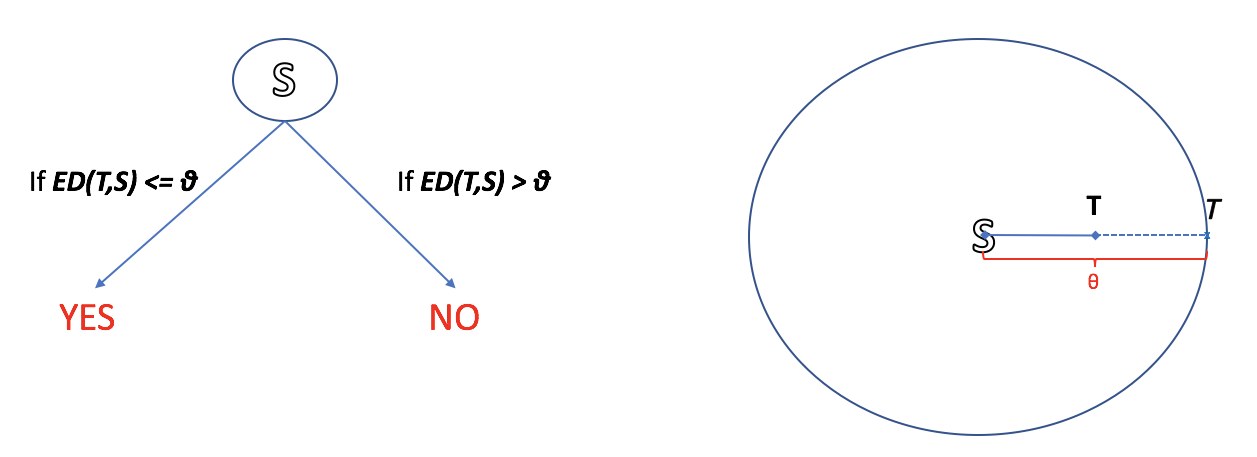
\includegraphics[scale=0.2]{exampleED.png}%
\caption{Example of time series tweaking under the ED.}\label{fig:exampleED}
\end{figure}

\section{Background}
\begin{definition} \textbf{($d$-dimensional time series)} %
A \emph{$d$-dimensional time series} $\mathcal{T} = \{\vec{T_{1}}, \ldots, \vec{T_{d}}\}$ is a sequence of $d$ variables, such that $\vec{T}_k\in \mathbb{R}^m$, $\forall k\in\{1,\dots,d\}$, where $\vec{T_k}=\{T_{k,1},\ldots,T_{k,m}\}$, with $T_{k,j}\in \mathbb{R}$, $\forall j\in\{1,\dots,m\}$. For $d=1$, $\mathcal{T}$ defines a \emph{univariate} time series, denoted simply as $\mathcal{T}=\{T_1,\ldots,T_m\}$ consisting of a sequence of $m$ ordered elements $T_j \in \mathbb{R}$. For $d>1$, $\mathcal{T}$ defines a \emph{multivariate} time series.
\end{definition}

A local segment of a time series is called a \emph{time series subsequence}. A more formal definition is given next.

\begin{definition} \textbf{(time series subsequence)} 
 A \emph{time series sub\-sequence} of the $k^{th}$ dimension of a time series $\mathcal{T}$ is a sequence of $l$ contiguous elements of $\vec{T}_k$, denoted as $\vec{T}_{k}^{s:s+l-1} = \{T_{k,s}, \ldots, T_{k,s+l-1}\}$, where $s$ is the starting position and $l$ is its length. Time series sub\-sequence and shapelet is used interchangeably.
\end{definition}

Time series classification predominantly relies on the chosen distance (similarity) measure to compare and discriminate between instance pairs. The main task is to employ a distance function $dist(\cdot)$ that compares two time series of equal length, and then given a time series subsequence (corresponding to a candidate discriminant shapelet) identify the closest subsequence match in the target time series. Depending on the application domain and the nature of the time series, various distance measures can be used.

\begin{definition} \textbf{(time series sub\-sequence distance)} 
Given a $1$-dimensional time series $\mathcal{S}$ and a $d$-dimensional time series $\mathcal{T}$ of lengths $l$ and $m$, respectively, such that $l \leq m$, the \emph{time series sub\-sequence distance} between $\mathcal{S}$ and the $k^{th}$ dimension of $\mathcal{T}$, is the minimum distance between $\mathcal{S}$ and any sub\-sequence of $\vec{T}_k$ of length $l$, i.e.:
\begin{equation}
  Sdist(\mathcal{S}, \vec{T}_k) = \min_{s=1}^{m-l+1} \{ 
  dist (\mathcal{S}, \vec{T}_k^{s:s+l-1}) \} \ .
\end{equation}
Note that since a $\mathcal{S}$ is $1$-dimensional time series of length equal to the length of each sub\-sequence $\vec{T}_k'^{s:s+l-1}$, dist can be applied directly.
\end{definition}

One possible distance function for $dist(\cdot)$ is the Euclidean distance.
\begin{definition} \textbf{(time series Euclidean distance)} %
Given two time series $\mathcal{T}$ and $\mathcal{T'}$ of equal length $l$, the distance between their corresponding $k^{th}$ dimensions is the length-normalized Euclidean distance between $\vec{T}_k$ and $\vec{T}_k'$, i.e.:
\begin{equation}
 dist(\vec{T}_k,\vec{T}_k') = ED (\vec{T}_k,\vec{T}_k') =  \sqrt{\frac{1}{l} \sum_{i=1}^{l}(T_{k,i}-T_{k,i}')^2} \ .
\end{equation}
 
\end{definition}
Finally, we define the distance between a time series sub\-sequence and a time series.

A collection of $n$ time series $\mathcal{D} = \{\mathcal{T}^{1},\ldots,\mathcal{T}^{n}\}$ defines a \emph{time series dataset}. 

\begin{definition} \textbf{(time series classification function)} %
  Given a dataset $\mathcal{D}$ of $n$ time series and a finite set of
  labels $\mathcal{C}$, a classification function is a mapping
  $f : \mathcal{D} \rightarrow \mathcal{C}$, such that for each
  $\mathcal{T}^{i}\in \mathcal{D}$

\[
f(\mathcal{T}^{i}) = \hat{y}_i\in \mathcal{C} \ ,
  \forall i\in \{1,\dots,n\} \ .
\]
\end{definition}

\subsection{Problem formulation}

Let $\mathcal{R} = \{F_1, \dots, F_k\}$ be a random shapelet forest, where each $F_i$ is a random shapelet tree. Consider a time series test example $\mathcal{T}$, and for simplicity let us focus on the univariate case. 

Suppose that the predicted class by $\mathcal{R}$ for $\mathcal{T}$ is $f(\mathcal{T}) = -1$, which also equals the actual class of $\mathcal{T}$. The objective is to identify those classifiers in $\mathcal{R}$ for which $h(\mathcal{T}) = -1$, i.e., those who disagree with the ensemble prediction. 

\section{Proposed Method}

\subsection{Decision stump}
The simplest problem in our setting is a decision stump. Given a decision node, a shapelet $\mathcal{S}$, a time series $\mathcal{T}$, and a matching threshold $\theta$, we can have two possible settings:
\begin{equation}
f(\mathcal{T}) = 
\begin{cases}
    1,& \text{if } Fdist(\mathcal{S}, \mathcal{T}) \leq \theta\\
    -1,              & \text{otherwise}
\end{cases}
\end{equation}

Or alternatively, 
\begin{equation}
f(\mathcal{T}) = 
\begin{cases}
    1,& \text{if } Fdist(\mathcal{S}, \mathcal{T}) > \theta\\
    -1,              & \text{otherwise}
\end{cases}
\end{equation}

\subsection{Generalization and overall algorithm}
The simplest problem in our setting is a decision stump.



\bibliographystyle{spbasic} 
\bibliography{references}


\end{document}
